\chapter{指数函数与对数函数}
\section{有理指数函数}
在本教材第三册中,已经把指数幂的定义范围从正整指
数逐步推广到“负整数”,“正、负分数”,在逐步推广过程
中,我们始终遵守的指导原则是保有指数法则:
\[a^m\cdot a^n=a^{m+n},\qquad  (a^m)^n=a^{m\cdot n}\]
指数在有理数系$\mathbb{Q}$内,我们有下面的指数幂的定义:
\[\begin{split}
  a^n=\underbrace{a\cdot a\cdot a\cdots a}_{\text{$n$个$a$}},&\qquad (n\in\mathbb{N})\\  
a^0=1,&\qquad (a\ne 0)\\  
a^{-n}=\frac{1}{a^n},&\qquad (a\ne 0)\\ 
a^{\tfrac{m}{n}}=\sqrt[n]{a^m}=\left(\sqrt[n]{a}\right)^m,&\qquad (a\ge 0,\; m,n\in\mathbb{N})\\ 
a^{-\tfrac{m}{n}}=\frac{1}{a^{\tfrac{m}{n}}},&\qquad (a> 0)\\ 
\end{split}\]
采用上面定义后,我们在第三册中也证明了正实数$a$和$b$的有
理指数幂依然满足指数运算法则:
\[a{\alpha}\cdot a^{\beta}=a^{\alpha+\beta},\qquad (a^{\alpha})^{\beta}=a^{\alpha\beta},\qquad (a\cdot b)^{\alpha}=a^{\alpha}\cdot b^{\alpha}\]
这里$\alpha,\beta \in \mathbb{Q}$。

这样一来,函数$a^x\; (a>0)$对于任意有理数$x$都有定义
了。我们称它为有理指数函数,这个函数具有上面所说的三
个性质。下面将进一步研讨这个函数的其它重要性质:

\begin{blk}{性质1}
\begin{enumerate}
    \item 若$a>1$, 当有理数$x>0$时,则$a^x>1$, 当有理
    数$x<0$时,则$a^x<1$。
    \item 若当$0<a<1$, 有理数$x>0$时,则$a^x<1$, 当有理数$x<0$
    时,则$a^x>1$。
\end{enumerate}
\end{blk}

\begin{proof}
\begin{enumerate}
\item 若$a>1$, 
\begin{enumerate}
  \item 设$x=\frac{m}{n}>0,\; (m,n\in\mathbb{N})$, 则$a^x=
a^{\tfrac{m}{n}}=\sqrt[n]{a^m}$, 因为$a>1$, 所以$a^m>1$ (幂函数$f(x)=x^m$在
$[0,+\infty)$上是严格递增的),又$\sqrt[n]{a^m}>1$ (幂函数$f(x)=x^{\tfrac{1}{n}}$
在$[0,+\infty)$上是严格递增的),即$a^x>1$.
\item 设$x<0$, 
$x=-x_1,\; (x_1>0)$,则$0<a^x=a^{-x_1}=\frac{1}{a^{x_1}}<1$,($\because\; a^{x_1}>1$)。
\end{enumerate}
 
\item 若$0<a<1$, 
\begin{enumerate}
  \item 设$a=\frac{1}{a_1},\; a_1>1$, 则当$x>0$, $a^x=\left(\frac{1}{a_1}\right)^x=\frac{1}{a^x_1}<1$, ($\because\; a_1^{x}>1$)。
  \item 设$x<0$, $x=-x_1,\; (x_1>0)$则
$a^x=a^{-x_1}=\frac{1}{a^{x_1}}>1$, ($\because\; a^{x_1}<1$)。
\end{enumerate}
\end{enumerate}
\end{proof}

性质1的几何意义表明:当$a>1$时,有理指数函数$y=
a^x$的图象上的点在有单斜线的区域I和II的部分;当$0<a<
1$时,$y=a^x$的图象上的点在有双斜线的区域III和IV的部分
(图6.1)。

\begin{figure}[htp]
  \centering
\begin{tikzpicture}[>=latex, scale=.7]
\draw[->] (-3,0)--(4,0)node[right]{$x$};
\draw[->] (0,-1)--(0,5)node[right]{$y$};
\node at (-.25,-.25){$O$};
\draw[very thick](-3,1)--(3.5,1)node[right]{$y=1$};
\fill[pattern = north east lines] (-3,1)  rectangle (0,0);
\fill[pattern = north east lines] (3,4.5)  rectangle (0,0);
\fill[pattern = crosshatch] (-3,4.5)  rectangle (0,1);
\fill[pattern = crosshatch] (3,1)  rectangle (0,0);

\end{tikzpicture}
  \caption{}
\end{figure}

\begin{blk}{性质2}
\begin{enumerate}
  \item 若$a>1$, $x_1<x_2$,则$a^{x_1}<a^{x_2}$, 即底数大于1的
有理指数函数$a^x$是递增的;
\item 若$0<a<1$, $x_1<x_2$,则$a^{x_1}>a^{x_2}$,即底数小于1的正数的有理指数函数$a^x$是递减的。
\end{enumerate}
\end{blk}

\begin{proof}
  若$a>1$和$x_1<x_2$, 那么
\[a^{x_2}-a^{x_1}=a^{x_1}\left(\frac{a^{x_2}}{a^{x_1}}-1\right)=a^{x_1}\left(a^{x_2-x_1}-1\right)\]
  
因为$x_2-x_1>0$, $a>1$, 所以$a^{x_2-x_1}>1$, 又$a^{x_1}>0$. 因
此,$a^{x_2-x_1}>0$, 即$f(x)=a^x,\; (a>1)$是递增的。

若$0<a<1$和$x_1<x_2$, 那么
\[a^{x_2}-a^{x_1}=a^{x_1}\left(a^{x_2-x_1}-1\right)\]
因为$x_2-x_1>0$, $0<a<1$, 所以$a^{x_2-x_1}<1$, 又$a^{x_1}>0$, 因
此$a^{x_2-x_1}<0$, 即$f(x)=a^x,\; (0<a<1)$是递减的。
\end{proof}

我们现在的任务是要把有理指数函数开拓为一个定义在
实数集上的连续函数。能否做到这一点的关键是如何对全体
无理点补充定义,使得指数函数在整个实数轴$\mathbb{R}$上处处连
续。为此,我们先说明有理指数函数的一个极限性质。


\begin{blk}{性质3}
  设$a>0$,则当$n\to +\infty$时,数列$\left\{a^{\tfrac{1}{n}}\right\}$的极限是1,即
  \[\lim_{n\to\infty}a^{\tfrac{1}{n}}=1\]
\end{blk}

\begin{proof}
\begin{enumerate}
  \item 当$a=1$时,结论自然成立。
  \item 当$a>1$时,因为
  $\frac{1}{n}>0$, 所以$a^{\tfrac{1}{n}}>1$ (性质1),
  设$a^{\tfrac{1}{n}}=1+h$, 其中$h>0$, 两边$n$次方,得到
 \[ a=(1+h)^n\]
 
 由贝努力不等式得
\[  a=(1+h)^n>1+nh\]
  所以,
$  0<h<\frac{a-1}{n},\qquad 1<1+h<1+\frac{a-1}{n}$,
  即:
\[1<a^{\tfrac{1}{n}}<1+\frac{a-1}{n}\]  
  再令$n\to +\infty$, 由上式就得到
\[1\le \lim_{n\to\infty}a^{\tfrac{1}{n}}\le 1 \]
  因此\[\lim_{n\to\infty}a^{\tfrac{1}{n}}=1\]
  \item 当$0<a<1$时,令$a=\frac{1}{b}$, 则$b>1$, 由上面的证明
  得到\[\lim_{n\to\infty}b^{\tfrac{1}{n}}=1\]
于是
\[\begin{split}
  \lim_{n\to\infty}a^{\tfrac{1}{n}}&=\lim_{n\to\infty}\left(\frac{1}{b}\right)^{\tfrac{1}{n}}=\lim_{n\to\infty}\frac{1}{b^{\tfrac{1}{n}}}\\
  &=\frac{1}{\displaystyle\lim_{n\to\infty}b^{\tfrac{1}{n}}}=\frac{1}{1}=1
\end{split}\]
\end{enumerate} 
\end{proof}

性质3可以进一步推广到下面的推论:

\begin{blk}{推论}
   若$a>0$且$a\ne 1$, 有理数数列$\{h_i\},\; i=1,2,3,\ldots$,
以0为极限,即$\Lim_{i\to\infty}h_i=0$, 那么
\[\lim_{i\to\infty}a^{h_i}=1\]
\end{blk}

\begin{proof}
  先设$a>1$, 因为$\Lim_{i\to\infty}h_i=0$, 必定存在这样的
自然数$N$, 使得当$i\ge N$时,$|h_i|<1$, 从而$\frac{1}{|h_i|}>1$。
用$m_i$表示$\left[\frac{1}{|h_i|}\right]$,
即不大于$\frac{1}{|h_i|}$
的最大整数,于是
\begin{equation}
  m_i=\left[\frac{1}{|h_i|}\right]\le \frac{1}{|h_i|}<m_i+1
\end{equation}
所以,当$i\ge N$时,有
\[\frac{1}{m_i+1}<|h_i|\le\frac{1}{m_i}\]
由$h\to 0$知,$\frac{1}{|h_i|}\to \infty$. 从而由$m_i+1>\frac{1}{|h_i|}$知,$m_i\to\infty$。根据有理指数幂的单调性,得
\[1<a^{|h_i|}<a^{\tfrac{1}{m_i}},\qquad (a>1)\]

仿照性质3的证明,令$b_i=a^{\tfrac{1}{m_i}}-1>0$, 于是,
\[\begin{split}
  a^{\tfrac{1}{m_i}}&=(1+b_i)\\
  a&=(1+b_i)^{m_i}>1+m_ib_i\\
  & 0<b_i<\frac{a-1}{m_i}
\end{split}\]
当$i\to 0$时,$m_i\to \infty$,

$\therefore\quad b_i\to 0$, 即$a^{h_i}\to 1$, 从而当$i\to \infty$时,$|h_i|\to 0$, $a^{|h_i|}\to 1$, 即$a^{h_i}\to 1$。

若$0<a<1$, 令$b=\frac{1}{a}>1$, 于是
\[\lim_{i\to \infty} a^{h_i}=\lim_{i\to \infty} \left(\frac{1}{b}\right)^{h_i}=\frac{1}{\Lim_{i\to \infty} b^{h_i}}=\frac{1}{1}=1\]
\end{proof}

应用这个推论,我们可以说明当有理数$x$的变化够小时,
有理指数函数$f(x)=a^x$的变化可以任意小。

\begin{blk}{性质4}
   当指数x的变化够小时,有理指数函数$f(x)=
a^x$的变化可以任意小。
\end{blk}

\begin{proof}
  设指数$x$从有理数$x_1$变化到有理数$x_2=x_1+h_i$,($h_i$
是有理数),且当$(x_2-x_1)\to 0$时,数列$\{h_i\}$以0为极限,于
是
\[\begin{split}
  \lim_{x_2\to x_1}\left(a^{x_2}-a^{x_1}\right)&=\lim_{i\to \infty}\left(a^{x_1+h_i}-a^{x_1}\right)\\
  &=a^{x_1}\cdot \lim_{i\to \infty}\left(a^{x_i}-1\right)=0
\end{split}\]
这就是说,只要$|h_i|$够小,那么$|a^{x_2}-a^{x_1}|$
就小于任意给定的正数$\varepsilon$.
\end{proof}


综合有理指数函数的性质,我们可以想象出$y=a^x\; (a>
1)$的图象如图10.2所示,但是我们不能用一条连续不断的
曲线把它画出来,因为指数$x$取无理数时,$a^x$还没有意义,
因而在有理指数函数的图象上,处处有空隙。下一节将由有理
指数函数的单调性和性质4, 适当给无理指数幂补充定义使
得指数函数在$\mathbb{R}$上处处连续。

\begin{figure}[htp]
  \centering
\begin{tikzpicture}[>=latex, scale=.7]
\draw[->] (-2,0)--(5,0)node[right]{$x$};
\draw[->] (0,-1)--(0,5)node[right]{$y$};
\node at (-.35,-.35){$O$};
\draw[dashed] (-2,1)--(4.5,1)node[right]{$y=1$};
\draw[domain=-2:3.5, samples=30, very thick, dashed]plot(\x, {1.6^(\x)});
\node at (0,1.3)[left]{$(0,1)$};
\node at (3,1.6^3)[right]{$y=a^x,\quad (a>1)$};
\end{tikzpicture}
  \caption{}
\end{figure}

\section*{习题10.1}
\addcontentsline{toc}{subsection}{习题10.1}
\begin{enumerate}
  \item 计算下列各式的值:
\begin{enumerate}
\item  $25^{3 / 2} \cdot 8^{4 / 3}$ 
\item $(0.09)^{1 / 2}+64^{2 / 3}+0.125^{2 / 3}-\frac{1}{16^{-3 / 2}}$
\item  $64^{1.5} \cdot(32)^{0.4} \div\left(\frac{9}{25}\right)^{-3 / 2}$
\item  $\left(\frac{81}{16}\right)^{-0.25}\left(5^{2}-0.1^{2} \cdot\left(\frac{1}{4}\right)^{-3}\right)^{2}$
\item  $\left[\frac{3}{9}-\left(\frac{2}{3}\right)^{-1}\right]^{-1}$
\item $(\sqrt{2})^{1.5}+\left(11+\frac{\sqrt[5]{5}}{5^{-0.8}}\right)^{-1 / 4}$
\item $\left[\left(\frac{3}{4}\right)^{0}\right]^{-0.5}-7.5(\sqrt{4})^{2}-(-2)^{-4}+81^{0.25}$
\item  $\left[\frac{1}{4}\left(0.027^{2 / 3}+15 \times 0.0016^{3 / 4}+1\right)\right]^{-1 / 2}$
\item  $6\left[\sqrt{3}\left(\sqrt{3}+2 \sqrt{2}+\frac{2}{3^{1 / 2}}\right)\right] \times\left(3^{1 / 2}+2^{1 / 2}\right)^{-2} \times\left(3^{-1}+2^{-1}\right)$
\item 若 $a=(2+\sqrt{3})^{-1},\quad  b=(2-\sqrt{3})^{-1}$, 计算 $(a+1)^{-1}+(b+1)^{-1}$
\end{enumerate}

\item  化简下列各式:
\begin{enumerate}
  \begin{multicols}{2}
\item  $b^{1 / 2} b^{1 / 3}$
\item  $b^{1 / 2} b^{-1 / 3}$
\item  $b^{-2 / 3} b^{3 / 5} ;$
\item  $b^{-2 / 3} b^{3 / 5} ;$
\item $\sqrt{a} \cdot \sqrt[3]{a} \cdot \sqrt[5]{a}$
\item  $\left[1-\left(a^{-1} b^{-1}\right)^{-1}\right]^{-2}$
\end{multicols}
\item  $\left[a^{-1 / 2} b^{-1 / 2}+a^{-1 / 6}\left(b^{-5 / 6}-a^{-1 / 3} b^{-1 / 2}\right)\right]^{-3 / 2}$
\item  $\frac{\left(a^{-1}+b^{-1}\right)(a+b)^{-1}}{\sqrt[6]{a^{4} \sqrt[5]{a^{-2}}}}$
\item  $\frac{a^{2}+a^{-2}-2}{a^{2}-a^{-2}}$
\item  $\left(a^{3 / 4}+b^{3 / 4}\right)\left(a^{3 / 4}-b^{3 / 4}\right) /\left(a^{1 / 2}-b^{1 / 2}\right)$
\item  $\left(e^{3 / 2}+2+e^{-3 / 2}\right)\left(e^{3 / 2}-2+e^{-3 / 2}\right)$
\item  $\left(a^{1 / 3}+a^{-1 / 3}\right)\left(a^{2 / 3}-1+a^{2 / 3}\right)$
\item  $\frac{m-n}{m^{1 / 2}-n^{1 / 2}}+\frac{m^{3 / 2}+n^{3/2}}{m^{1 / 2}+n^{1 / 2}}$
\item  $\frac{x^{2 p(q+1)}-y^{2 q(p-1)}}{x^{p(q+1)}-y^{q(p-1)}}$
\item  $\left(a^{4 / 3}-2+a^{-4 / 3}\right)\left(a^{2 / 3}-a^{-2 / 3}\right)$
\item  $\frac{m-n}{m^{1 / 2}-n^{1 / 2}}+\frac{m^{3 / 2}+n^{3/2}}{m^{1 / 2}+n^{1 / 2}}$
\item  $\left[\frac{4 a-9 a^{-1}}{2 a^{1 / 2}-3 a^{-1 / 2}}+\frac{a-4+3 a^{-1}}{a^{1 / 2}-a^{-1 / 2}}\right]^{2}$
\end{enumerate}

\item  解下列各方程:
  \begin{enumerate}
    \begin{multicols}{2}
  \item  $\sqrt{2 x-3}=4-x$
  \item  $\sqrt{2 x+8}+\sqrt{x+5}=7$
  \item  $x^{-1 / 4}+x^{-1 / 2}-6=0$
  \item  $x^{1 / 2}+x^{-1 / 2}-\frac{10}{3}=0$
\end{multicols}
  \item  $\sqrt[n]{(x+1)^{2}}+\sqrt[n]{(x-1)^{2}}=4 \sqrt[n]{x^{2}-1}$
\end{enumerate}

\item  设 $h_{i}=\frac{100}{2 i+1},\quad  m_{i}=\left[\frac{1}{h_{i}}\right]=\left[\frac{2 i+1}{100}\right]$
\begin{enumerate}
  \item 求证数列$\{h_i\}=\left\{\frac{100}{2 i+1}\right\}$递减,并求使$h_i=\frac{100}{2i+1}<1$的$i$的范围;
  \item 当$i=10,49,50,100,1000$时,求$m_i$的值;
  \item 求证当$i\ge 50$时,不等式$1<100^{\tfrac{100}{2i+1}}<100^{\tfrac{1}{m_i}}$成立;
  \item 求证:$\Lim_{i\to\infty}\left(100^{\tfrac{1}{m_i}}-1\right)=0,\quad \Lim_{i\to\infty}100^{h_i}=1$。
\end{enumerate}
\end{enumerate}

\section{无理指数幂的定义}
要把指数幂的定义由有理数推广到实数,自然又得用逼
近法。

设$\beta$是一个无理数,我们可以用两个有理数列$\{r_n\}$, $\{s_n\}$
去左、右夹逼,即$r_n\to \beta\leftarrow s_n$, 从而$\Lim_{n\to\infty}r_n=\Lim_{n\to\infty}s_n=\beta$. 现在
的问题是数列$\{a^{r_n}\}$,$\{a^{s_n}\}$,(这里$a>0$)的极限是否存
在?如果存在的话,我们就可以定义
\[a^{\beta}=\Lim_{n\to\infty}a^{r_n}=\Lim_{n\to\infty}a^{s_n}\]

从而就可以把有理指数函数$a^x$开拓为在$\beta$点连续的函数:
\[a^x\; (a>0,\; x\in \mathbb{Q}\cup\{\beta\})=\begin{cases}
  a^x\;  (x\in\mathbb{Q})\\
  a^{\beta}=\Lim_{n\to\infty}a^{r_n}=\Lim_{n\to\infty}a^{s_n}
\end{cases}\]

\begin{blk}{引理}
   设 $r_{n} \rightarrow \beta \leftarrow s_{n}$, 则
\begin{enumerate}
  \item 当$a>1$时,$a^{r_1}\le a^{r_2}\le \cdots\le a^{r_n}\le \cdots \le a^{s_n}\le \cdots\le a^{s_2}\le a^{s_1}$,且$\left(a^{r_n}-a^{s_n}\right)\to 0$
 
  当$0<a<1$时,$a^{r_1}\ge a^{r_2}\ge \cdots\ge a^{r_n}\ge \cdots \ge a^{s_n}\ge \cdots\ge a^{s_2}\ge a^{s_1}$,且$\left(a^{r_n}-a^{s_n}\right)\to 0$

  \item $\lim a^{r_n}=\lim a^{s_{n}}=A$ (即极限存在) 
\end{enumerate}
\end{blk}

\begin{proof}
  $a>1$和$0<a<1$这两种情形是完全相似的,只是
不等式方向反过来罢了,所以下面只讨论$a>1$的情形,
($a=1$时它的任何方幂都是1, 所以$1^{\beta}=1$)。我们只需
证明下述两点:
\begin{enumerate}
  \item $a>1$, $s>r$时,则$a^s>a^r$,(性质2)。
  \item $\because\quad $当$n\to\infty$时,$s_n-r_n=h_n\to 0$,
  
  $\therefore\quad $由性质4得
\[  a^{s_n}-a^{r_n}\to 0\]
  由实数完备性,存在一个唯一实数
 \[ A=\lim a^{s_n}=\lim a^{r_n}\]
\end{enumerate}
\end{proof}

\begin{blk}{定义}
  设$\beta$是一任意无理数,$r_n\to\beta\leftarrow s_n$是$\beta$的左、右夹
逼数列,并且$u>0$, 则定义
\[a^{\beta}=\lim a^{r_n}=\lim a^{s_n}\]
\end{blk}


我们要说明这个定义的合理性,即上述定义和$\beta$的夹逼有
理数列的选取无关。

设$r'_n\to\beta\leftarrow s'_n$是另外一对夹逼数列,则
\[r'_n\to\beta \leftarrow s_n,\qquad r_n\to\beta\leftarrow s'_n\]

由上述引理就有
\[\lim a^{r'_n}=\lim a^{s_n}=\lim a^{r_n}=\lim a^{s'_n}\]

在实数轴$\mathbb{R}$上,对每一个无理点,都补充这样的定义,
于是我们就把有理指数函数开拓为一个在实数轴上处处有定
义的指数函数$a^x,\; (a>0,\; x\in\mathbb{R})$。

下面我们将证明这样定义的无理指数幂仍满足指数
法则。

\begin{blk}{定理}
  指数法则$a^{\beta}\cdot a^{\gamma}=a^{\beta+\gamma}$, $\left(a^{\beta}\right)^{\gamma}=a^{\beta\cdot \gamma}$, $(ab)^{\beta}=a^{\beta}\cdot b^{\beta}$对于任何实数$\beta$, $\gamma$都成立。
\end{blk}
 
\begin{proof}
当$\beta$, $\gamma$是有理数时,上述等式已在本教材第三册
第一章给出证明,所以我们只要说明$\beta$, $\gamma$是无理数的情形。

设$r_n\to\beta\leftarrow s_n$, $c_n\to\gamma\leftarrow d_n$分别是$\beta$, $\gamma$的左、右夹逼数列,于是
\[(r_n+c_n)\to \beta+\gamma \leftarrow (s_n+d_n)\]
\[\begin{split}
  a^{\beta+\gamma}&=\lim a^{r_n+c_n}=\lim a^{r_n}\cdot a^{c_n}\\
  &=\lim a^{r_n}\cdot \lim a^{c_n}=a^{\beta}a^{\gamma}
\end{split}\]

现在让我们来证明$(a^{\beta})^{\gamma}=a^{\beta\cdot \gamma}$(为了讨论的方便,我们
只讨论$a>1,\; \beta ,\gamma>0$的情形),

设$r_n\to \beta \leftarrow s_n,\quad c_n\to \gamma\leftarrow d_n$,$r_n, s_n,c_n,d_n>0$, 则有
\[r_n\cdot c_n\to \beta_{\gamma}\leftarrow s_n\cdot d_n\]
根据正分指数的幂函数与有理指数函数的单调性有
\[(a^{r_n})^{c_n}<(a^{\beta})^{c_n}<(a^{\beta})^{\gamma}<(a^{\beta})^{d_n}<(a^{s_n})^{d_n}\]
所以由有理指数法则,得到
\[a^{r_n\cdot c_n}=(a^{\beta})^{c_n}<(a^{\beta})^{\gamma}<(a^{s_n})^{d_n}=a^{s_n\cdot d_n}\]
\[60+(u,.u,p-pus)\]
$\therefore\quad $由引理知,存在唯一的极限
\[(a^{\beta})^{\gamma}=\lim a^{r_n\cdot c_n} =\lim a^{s_n\cdot d_n} =a^{\beta\cdot \gamma}\]

最后证明:$(ab)^{\beta}=a^{\beta}\cdot b^{\beta}$, 只讨论$a>1$, $b>1$的情形。

$\because\quad a>1,b>1$

$\therefore\quad ab>1$, 于是
\[a^{r_n}b^{r_n}=(ab)^{r_n}<(ab)^{\beta}<(ab)^{s_n}=a^{s_n}b^{s_n}\]
\[(ab)^{s_n}-(ab)^{r_n}\to 0\]
因此,$(ab)^{\beta}=\lim a^{r_n}b^{r_n} = \lim a^{r_n}\cdot \lim b^{r_n}=a^{\beta}\cdot b^{\beta}$
\end{proof}

\begin{example}
  \begin{enumerate}
    \item $10^{\sqrt{2}}\cdot 10^{\sqrt{3}}=10^{\sqrt{2}+\sqrt{3}}$
    \item  $\left[\left(\sqrt[3]{2}\right)^{\sqrt{8}}\right]^{\tfrac{\sqrt{2}}{2}}=2^{\tfrac{1}{3}\x 2\sqrt{2}\x\tfrac{\sqrt{2}}{2}}=2^{\tfrac{2}{3}}=\sqrt[3]{4}$
    \item $\left(5^{-\sqrt{2}}a^{\sqrt{8}}b^{\tfrac{\sqrt{2}}{2}}\right)^{\tfrac{\sqrt{2}}{2}}=5^{-1}a^{2}b^{\tfrac{1}{2}} =\frac{a^2\sqrt{b}}{5} $
  \end{enumerate}
\end{example}

\section{实指数函数}
总结上节推广的结果,就得到一个对任意实数$x$都有定
义的\textbf{实指数函数}:
\[f:\mathbb{R}\mapsto \mathbb{R}^+,\qquad \text{这里} f(x)=a^x,\; (a>0, \; \text{且}a\ne 1)\]

这个函数就叫做\textbf{以$a$为底的指数函数}。上节还说明了指
数函数是一个满足下面两个性质的连续函数:
\begin{enumerate}
  \item $f(x_1+x_2)=a^{x_1+x_2}=a^{x_1}\cdot a^{x_2}=f(x_1)\cdot f(x_2)$
  \item $f(kx)=a^{kx}=(a^x)^k=[f(x)]^k$
\end{enumerate}

现在,我们还须验证实指数幂保有有理指数幂的一切性
质,并且实指数函数是连续的。

\begin{blk}{性质1}
\begin{enumerate}
  \item 若$a>1$, 当$x>0$时,则$a^x>1$;
当$x<0$时,则$a^x<1$.
\item 若$0<a<1$, 当$x>0$时,则$a^x<1$; 
当$x<0$时,则$a^x>1$.
\end{enumerate}
\end{blk}

\begin{proof}
  如果$x$是有理数,我们在第一节中给过证明,这里不
再重述,所以我们只要证明$x$是无理数的情形,设$x>0$,
且$c_n\to x\leftarrow d_n$是$x$的有理数夹逼数列。在数列$\{c_n\}$中一定存在
某一项$c_N$和它后面的一切项都是正数,不然的话,如果对于
所有的$n$, 有$c_n\le 0$, 于是$\lim c_n\le 0$即$x\le 0$, 这和已知的$x>0$
矛盾。

令$c_N>0$, 则$a^{C_N}>a^0=1$, 而$a^x>a^{c_N}>1$, 这就证明了
$a^x>1$.

设$x<0$, $x=-y$, 则$y>0$, $a^x=a^{-y}=\frac{1}{a^y}$

$\because\quad a^y>1,\qquad \therefore\quad a^x=\frac{1}{a^y}<1$

$0<a<1$的情形,留给同学证明。
\end{proof}

\begin{blk}{性质2}
\begin{enumerate}
  \item 若$a>1$且$x_2>x_1$, 则$a^{x_2}>a^{x_1}$
  \item 若$0<a<1$且$x_2>x_1$, 则$a^{x_2}<a^{x_1}$
\end{enumerate}
\end{blk}

\begin{proof}
设$a>1$且$x_2>x_1$,
\[a^{x_2}-a^{x_1}=a^{x_1}\left(a^{x_2-x_1}-1\right)\]
因为$x_2-x_1>0$, 于是$a^{x_2-x_1}>1$, 因此$a^{x_2}-a^{x_1}>0$.

设$0<a<1$ 且$x_2>x_1$,
\[a^{x_2}-a^{x_1}=a^{x_1}\left(a^{x_2-x_1}-1\right)\]
因为$x_2-x_1>0$, 则$a^{x_2-x_1}<1$, 因此$a^{x_2}-a^{x_1}<0$.  
\end{proof}

\begin{blk}{性质3}
\[\lim_{x\to 0} a^x=1\]
\end{blk}


对这个极限的证明可以仿照第一节中性质3的推论的证法
去证。利用性质3, 容易证明实指数函数处处连续。

\begin{blk}{性质4}
当$x$无限增大时,$a^x,\; (a>1)$也无限增大,可以写
成$\Lim_{x\to\infty} a^x=+\infty$ (注意这个表达式并不表示此极限存在,而是
说$a^x$可以超过任何一个指定的正数),若$0<a<1$, 则
$\Lim_{x\to\infty} a^x=0$
\end{blk}

\begin{proof}
  为确定起见,设$a>1$, 令$a=1+h\; (h>0)$, 因为
\[(1+h)^n>1+nh,\qquad (n\in\mathbb{N})\]
可得:$a^n>1+n(a-1)$。

对于任意给定的一个正数$M$, 当$n>\frac{M-1}{a-1}$时,则
\[a^n>1+n(a-1)>1+\frac{M-1}{a-1}(a-1)=M\]
所以,当$x>n$时,便有$a^x>a^n>M$。

这就是说,当$x\to +\infty$时,$\lim a^x=\infty$.

设$0<a<1$, $a=\frac{1}{b}$, 则$b>1$, $a^x=\left(\frac{1}{b}\right)^n=\frac{1}{b^n}$,
任给$\varepsilon=\frac{1}{M}>0$, 则$M=\frac{1}{\varepsilon}$, 依前段,当$x>n>\frac{M-1}{a-1}$时,有$b^x>M$. 于是$a^x=\frac{1}{b^x}<\frac{1}{M}=\varepsilon$. 这就证明了当$x\to\infty$时,$\lim a^x=0,\; (0<a<1)$.
\end{proof}

\begin{blk}{性质5}
\begin{enumerate}
  \item 若$a>1$, $\Lim_{x\to-\infty} a^x=0$.
  \item 若$0\le a<1$, $\Lim_{x\to-\infty} a^x=+\infty$.
\end{enumerate}  
\end{blk}

\begin{proof}
为确定起见,设$a>1$, 令$x=-y,\; (y>0)$,则当
$x\to-\infty$时,$y\to +\infty$, 所以
\[\Lim_{x\to-\infty} a^x=\Lim_{y\to +\infty} a^{-y}=\Lim_{y\to +\infty}\frac{1}{a^y}=\frac{1}{\Lim_{y\to +\infty}a^y}=0\]

$0<a<1$的情形,证明留给读者。
\end{proof}

总结上面的讨论,指数函数有下面的主要性质:

\begin{blk}{定理}
   指数函数$f:(-\infty,+\infty)\mapsto (0,+\infty)$, 这里$f(x)=a^x,\; (a>0\text{\; 且\; }a=1)$, 满足下列三个性质:
\begin{enumerate}
  \item $f(x_1+x_2)=f(x_1)f(x_2)$
  \item $f(x)$是严格单调的,$a>1$时,递增;$0<a<1$时,递减
  \item $f(x)$是连续的
\end{enumerate}
\end{blk}

指数函数的图象如图10.3所示:
\begin{figure}[htp]
  \centering
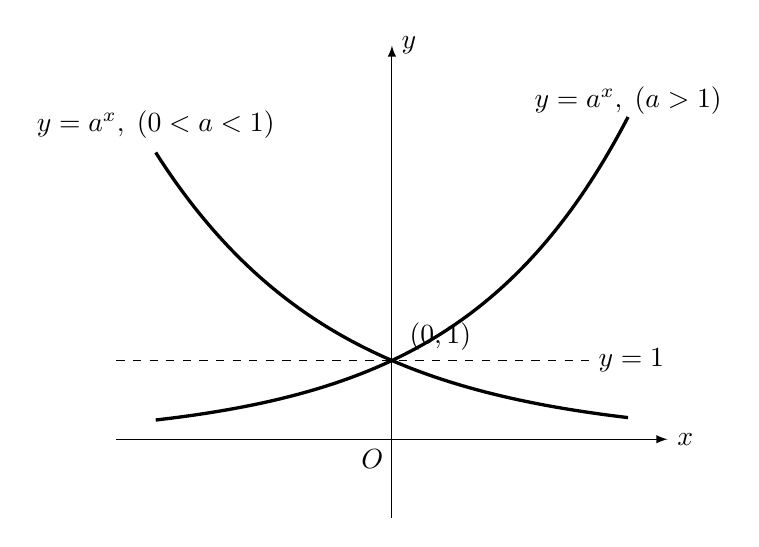
\begin{tikzpicture}[>=latex]
\draw[->](-3.5,0)--(3.5,0)node[right]{$x$};
\draw[->](0,-1)--(0,5)node[right]{$y$};
\draw[dashed] (-3.5,1)--(2.5,1)node[right]{$y=1$};
\draw [domain=-3:3, samples=100, very thick]plot(\x, {1.6^(\x)});
\draw [domain=-3:3, samples=100, very thick]plot(\x, {0.65^(\x)});
\node at (-3,4){$y=a^x,\; (0<a<1)$};
\node at (3,4.3){$y=a^x,\; (a>1)$};
\node at (-.25,-.25){$O$};
\node at (.1,1.3)[right]{$(0,1)$};
\end{tikzpicture}
  \caption{}
\end{figure}

\begin{blk}{逆定理}
  任何一个满足上述性质1和2的函数
$f(x)$必定是一个指数函数,其底为$a=f(1)$。
\end{blk}
 
\begin{proof}
由性质1, 对于任何实数$x$, 有
\[f(0)f(x)=f(0+x)=f(x)\]
即得,$f(0)=1$. 当$f(x)$递增时,$f(1)=a>f(0)=1$, 而当
$f(x)$递减时,$f(1)=a<f(0)=1$.

由性质1:
\[\begin{split}
  f(m)&=f\big((m-1)+1\big)=f(m-1)\cdot f(1)\\
  &=f(m-2)\cdot \big(f(1)\big)^2=f(m-3)\cdot \big(f(1)\big)^3\\
\cdots & \cdots \cdots \cdots \cdots \\
&=\big(f(1)\big)^m=a^m
\end{split}\]
又因为
\[\begin{split}
  \left[f\left(\frac{m}{n}\right)\right]^n&=f\overbrace{\left(\frac{m}{n}+\frac{m}{n}+\cdots +\frac{m}{n}\right)}^{n\text{个}}\\
  &=f(m)=a^m
\end{split}\]
所以:$f\left(\frac{m}{n}\right)=\sqrt[n]{a^m}=a^{\tfrac{m}{n}}$

因为$f\left(\frac{m}{n}\right)f\left(-\frac{m}{n}\right)=f\left(\frac{m}{n}-\frac{m}{n}\right)=f(0)=1$

所以$f\left(-\frac{m}{n}\right)=\frac{1}{f\left(\frac{m}{n}\right)}=\frac{1}{a^{\tfrac{m}{n}}}=a^{-\tfrac{m}{n}}$

所以,$f(r)=a'$, 对于正、负分数$r$都成立。

再由单调性,和实指数幂的定义,就可以说明$f(x)=a^x$
对于任何实数都成立。

设$x\in\mathbb{R}$为一任意实数,$r_n\to x\leftarrow s_n$是$x$的左、右夹逼有理
数列,即
\begin{equation}
  r_1\le r_2\le \cdots \le r_n\le \cdots \le x\le \cdots \le s_n\le \cdots \le s_2\le s_1
\end{equation}
并且 $\lim(s_n-r_n)=0$.

由不等式(10.2)和$f(x)$的递增性(递减性),得到
\begin{equation}
  f(r_1)\le f(r_2)\le \cdots \le f(r_n)\le \cdots \le f(x)\le \cdots \le f(s_n)\le \cdots \le f(s_2)\le f(s_1)
\end{equation}
$r_n,s_n$都是有理数。
(若$f(x)$递减,我们得到不等式(10.3)的反向不等式)。

不等式(10.3)可改写成
\begin{equation}
  a^{r_1}\le a^{r_2}\le \cdots \le a^{r_n}\le \cdots \le a^{x}\le \cdots \le a^{s_n}\le \cdots \le a^{s_2}\le a^{s_1}
\end{equation}
而上节实数指数定义中,$a^x$是唯一能满足(10.4)的实数,所以$f(x)=a^x$。

在上面的讨论中,$x$是一个任意的实数,因此,$f(x)=
a^x$, 对于任何实数$x$恒成立。
\end{proof}

\begin{example}
    设$a,b$是不等的正实数,试证
\[  a^ab^b>(ab)^{\tfrac{a+b}{2}}>a^bb^a\]
\end{example}

\begin{proof}
  不妨设$a>b$, 则$\frac{a}{b}>1$, $a-b>0$.
  于是,根据实指数幂性质1,可得:
\[\frac{a^ab^b}{(ab)^{\tfrac{a+b}{2}}}=a^{\tfrac{a-b}{2}}\cdot b^{\tfrac{b-a}{2}}=\left(\frac{a}{b}\right)^{\tfrac{a-b}{2}}>1\]

  由于$a>0,\;  b>0\Rightarrow ab>0$, 因此,$(ab)^{\tfrac{a+b}{2}}>0$, 所
  以,有
\[  a^ab^b>(ab)^{\tfrac{a+b}{2}}\]
  另外,根据同样的道理,有
\[\frac{(ab)^{\tfrac{a+b}{2}}}{a^bb^a}=a^{\tfrac{a-b}{2}}\cdot b^{\tfrac{b-a}{2}}=\left(\frac{a}{b}\right)^{\tfrac{a-b}{2}}>1\]
  又$a^b>0$, $b^a>0$. 所以$(ab)^{\tfrac{a+b}{2}}>a^b b^a$, 这就证明了
  \[a^ab^b>(ab)^{\tfrac{a+b}{2}}>a^b b^a\]
\end{proof}

\section*{习题10.2}
\addcontentsline{toc}{subsection}{习题10.2}
\begin{enumerate}
  \item 利用实指数幂的性质,指出下列不等式中,$a$是大
  于1, 还是大于0而小于1?
\begin{multicols}{2}
  \begin{enumerate}
  \item $a^{\sqrt{2}}<a^{\tfrac{\sqrt{2}}{2}}$
  \item $a^{-\sqrt{3}}>a^2$
  \item $a^{-\sqrt{5}-\sqrt{7}}>a^{-5}$
  \item $a^{1+\sqrt{5}}<a^{2+\sqrt{2}}$
  \item $a^{\sqrt{7}+\sqrt{2}}<a^{\sqrt{6}+\sqrt{3}}$
\end{enumerate}
\end{multicols}

\item 作下列各函数的图象:
\begin{multicols}{2}
  \begin{enumerate}
  \item $y=3^x$
  \item $y=3^{-x}$
\end{enumerate}
\end{multicols}

\item \begin{enumerate}
  \item 证明$f(x)=\frac{2^x+2^{-x}}{2}$是偶函数,并作出它的图象;
  \item 当$x$为何值时,$f(x)$有最小值,并求最小值。
\end{enumerate}

\item 设$a,b,c$是不等的正数,证明:
\begin{enumerate}
  \item $a^{2 a} b^{2 b} c^{2 c}>a^{b+c} b^{c+a} c^{a+b}$
  \item $a^{a} b^{b} c^{c}>(a b c)^{\tfrac{a+b+c}{3}}$
\end{enumerate}
(提示:利用例10.2的结果)

\item 证明:
\begin{enumerate}
  \item 当$n$是1或不小于5的自然数时,总有$2^n>n^2$;
  \item $\Lim_{n\to\infty}\frac{2^n}{n}=\infty$。
\end{enumerate}
\end{enumerate}

\section{对数函数}

由实数幂的定义,我们得知指数函数
\[a^x,\quad (a>0,\;a\ne 1),\qquad x\in\mathbb{R}\]
的值都是正的,现在还要进一步说明指数函数的值域是正实
数集,也就是必须证明下面的命题。

\begin{blk}{命题}
   给定不等于1的正实数$a$, 对于任意正数$b$, 一
定存在唯一的一个实数$c$, 满足下列方程
$$a^c=b$$
\end{blk}

\begin{proof}
  为确定起见,设$a>1$, 依实指数函数的性质5,
$\Lim_{x\to-\infty}a^x=0$, 可以找出这样一数$c_1$以使$a^{c_1}<b$, 依$a^x,\;(a>1)$
是增函数且$\Lim_{x\to+\infty}a^x=+\infty$, 可以找出这样的数$c_2>c_1$, 以使
$a^{c_2}>b$, 现在由连续函数中间值定理知道,在$c_1$与$c_2$之间有
实数$c$以使$a^c=b$, 再由单调性知道这个数是唯一的。类似
地可以证明$0<a<1$的场合,这个证明留给同学补全。
\end{proof}


现在我们根据第八章第五节反函数定理可以说由指数函数
得到一个定义在正实数变域上的反函数,称为对数函数,记
作$f:\mathbb{R}^+\mapsto \mathbb{R}$, 这里$f(x)=\log_a x$, 它是连续的单调函数。正式定义如下:

\begin{blk}{定义}
   若$a>0$且$a\ne 1$, 那么$y=\log_a x$, 当且仅当
$x=a^y$. 我们称$y$是以$a$为底的对数,函数$f:\mathbb{R}^+\mapsto \mathbb{R}$,这里
$f(x)=\log_a x$称为\textbf{对数函数}。
\end{blk}

这个定义导致下面有用的结果:
\begin{enumerate}
  \item $a^{\log_a x}=x,\qquad \log_a a^x=x$
  \item $\log_a (xy)=1ogax+\log_a y$
  \item $\log_a \frac{x}{y}=\log_a x-\log_a y$
  \item $\log_a x^r=r\log_a x$
  \item $\log_a b=\frac{\log_c b}{\log_c a}$(换底公式)。
\end{enumerate}
证明过程请看第三册第一章。

从函数的图象来说:$y=\log_a x,\; (x\in\mathbb{R})$的图象能由$y=a^x,\; (x\in\mathbb{R})$的图象经$y=x$的反射而得到,如图10.4。
\begin{figure}[htp]
  \centering
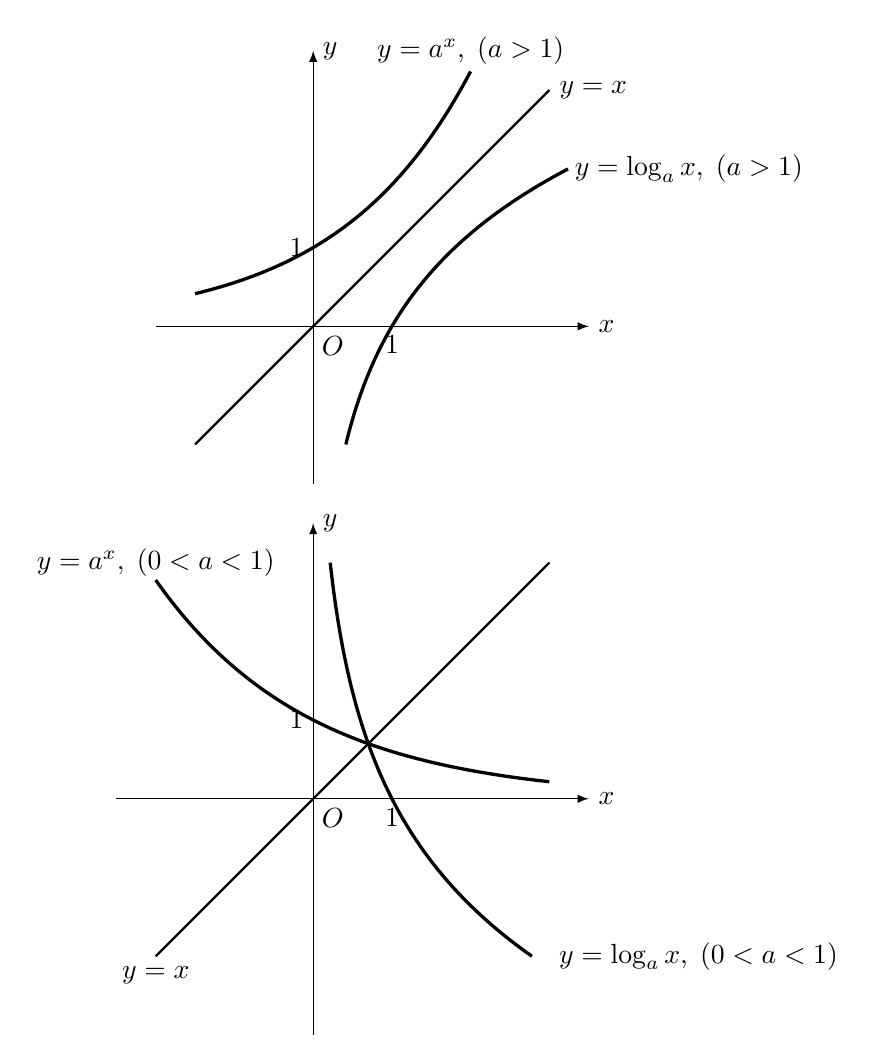
\begin{tikzpicture}[>=latex]
\begin{scope}
  \draw[->](-2,0)--(3.5,0)node[right]{$x$};
\draw[->](0,-2)--(0,3.5)node[right]{$y$};
\draw[thick] (-1.5,-1.5)--(3,3)node[right]{$y=x$};
\draw[domain=-1.5:2, samples=100, very thick]plot(\x,{1.8^(\x)});
\draw[domain=-1.5:2, samples=100, very thick]plot({1.8^(\x)},\x);
\node at (2,3.5){$y=a^x,\; (a>1)$};
\node at (3.2,2)[right]{$y=\log_a x,\; (a>1)$};
\node at (1,0)[below]{1};
\node at (0,1)[left]{1};
\node at (.25,-.25){$O$};
\end{scope}
\begin{scope}[yshift=-6cm]
  \draw[->](-2.5,0)--(3.5,0)node[right]{$x$};
  \draw[->](0,-3)--(0,3.5)node[right]{$y$};
  \draw[thick] (-2,-2)node[below]{$y=x$}--(3,3);
  \draw[domain=-2:3, samples=100, very thick]plot(\x,{0.6^(\x)});
  \draw[domain=-2:3, samples=100, very thick]plot({0.6^(\x)},\x);
  \node at (-2,3){$y=a^x,\; (0<a<1)$};
\node at (3,-2)[right]{$y=\log_a x,\; (0<a<1)$};
\node at (1,0)[below]{1};
\node at (0,1)[left]{1};
\node at (.25,-.25){$O$};
\end{scope}
\end{tikzpicture}
  \caption{}
\end{figure}

由于$x$轴是指数函数图象的渐近线,故$y$轴是对数函数
图象的渐近线。相应于指数函数的极限值:
\[\begin{split}
  \lim_{x\to -\infty} a^x=0&,\qquad a>1\\
  \lim_{x\to +\infty} a^x=0&,\qquad 0<a<1
\end{split}\]
有对数函数的极限值:
\[\lim_{x\to 0^+} \log_a x=\begin{cases}
  -\infty, & a>1\\
  +\infty ,& 0<a<1
\end{cases}\]

相应于指数函数的特征性质,也就有对数函数的特征
性质:
\begin{enumerate}
  \item $\log_a (x_1\cdot x_2)=\log_a x_1+\log_a x_2$
  \item 单调性。当$a>1$递增;当$0<a<1$递减。
  \item 连续性。即在$(0,+\infty)$内处处连续。同样地,对
  应于第三节中的定理,总结成下面的定理。
\end{enumerate}

\begin{blk}{定理}
  对数函数$f(x)=\log_a x$满足下列性质:
  \begin{enumerate}
    \item $f(x_1\cdot x_2)=f(x_1)+f(x_2)$
    \item 单调性。$a>1$时,递增;$0<a<1$时,递减。
    \item 在$x>0$半直线上,处处连续。
  \end{enumerate}
\end{blk}
 
\begin{blk}{逆定理} 
  任何一个满足性质1、2的函数$f(x)$一
定是一个对数函数,即存在适当的$a$, 使得$f(x)=\log_a x$.
\end{blk}

\begin{proof}
  由性质1,$f(x_1)=f(x_1\cdot 1)=f(x_1)+f(1)$。
因此$f(1)=f(x_1)-f(x_2)=0$.

我们先任取一常数$A>1$, 则由性质2知
\[f(A)\ne f(1)=0\]
再由性质1
\[f(A^m)=\underbrace{f(A)+f(A)+\cdots+f(A)}_{\text{$m$项}}=mf(A),\qquad m\in\mathbb{N}\]

又
\[\begin{split}
  mf(A)&=f(A^m)=f\left(\left((A)^{\tfrac{m}{n}}\right)^n\right)\\
  &=\underbrace{f\left(A^{\tfrac{m}{n}}\right)+\cdots+f\left(A^{\tfrac{m}{n}}\right)}_{\text{$n$项}}=nf\left(A^{\tfrac{m}{n}}\right)
\end{split} \]
$\therefore\quad f\left(A^{\tfrac{m}{n}}\right)=\frac{m}{n}f(A),\qquad m,n\in\mathbb{N}$

又$\because\quad f\left(A^{\tfrac{m}{n}}\right)+f\left(A^{-\tfrac{m}{n}}\right)=f\left(A^{\tfrac{m}{n}}\cdot A^{-\tfrac{m}{n}}\right)=f(A^0)=f(1)=0$

$\therefore\quad f\left(-A^{\tfrac{m}{n}}\right)=-f\left(A^{\tfrac{m}{n}}\right)=-\frac{m}{n}f(A)$

综合上面所证,所以对于所有有理数$r\in\mathbb{Q}$, 都有
\[f(A^r)=rf(A)\]
从此不难用单调性和极限过程,导出
\begin{equation}
  f(A^{\beta })=\beta f(A),\qquad \beta \in\mathbb{R}
\end{equation}

令$A^{\beta }=x$, 则$\beta =\log_A x$, 于是(10.5)可写成
\begin{equation}
  f(x)=f(A)\cdot \log_A x
\end{equation}
这样我们得到一个连续的单调的对数型函数(10.6). 为了化去
常数因子$f(A)$, 我们要用一些技巧如下:令$a=A^{\tfrac{1}{f(A)}}$
, 于是
\[1=\log_a a=\log_a A^{\tfrac{1}{f(A)}}=\frac{1}{f(A)}\cdot \log_a A\]
即:$f(A)=\log_a A$, 代入(10.6), 得到:
\[f(x)=\log_A x\cdot \log_a A=\log_a x\]
\end{proof}

\section*{习题10.3}
\addcontentsline{toc}{subsection}{习题10.3}
\begin{enumerate}
  \item 求下列各函数的定义域与值域,如果它们是可逆的,
  写出以$x$为自变数的反函数。
  \begin{multicols}{2}
    \begin{enumerate}
      \item $y=\log_2(x-2)$
      \item $y=\log_2\frac{1}{x}$
      \item $y=e^{-x}$
      \item $y=\sqrt{\lg\cos2\pi x}$
    \end{enumerate}
  \end{multicols}

  \item 计算下列各式的值:
\begin{multicols}{2}
\begin{enumerate}
  \item $2^{\log_4 9}$
  \item $5^{\log_{0.2} 7}$
  \item $3^{\log_{\sqrt{2}}6}$
  \item $6^{1+\log_6 5}$
  \item $25^{\tfrac{1}{3} \log 5^{27}-\log_{5} 4}$
  \item $10^{\lg\sqrt{100}}$
  \item $\log _{\sqrt{4-\sqrt{15}}} \sqrt{4+\sqrt{15}}$
  \item $4-\lg 8-3 \lg 5$
  \item $ \lg ^{2} 5+\lg 2 \lg 50$
  \item $\frac{3 \lg 1728}{1+\frac{1}{2} \lg 0.36+\frac{1}{3} \lg 8}$
  \item $\log _{a} b \cdot \log _{b} c \cdot \log _{c} d$
  \item $\left(\log _{2} 3+\log _{4} 9\right)\left(\log _{3} 4+\log _{9} 2\right)$
\end{enumerate}
\end{multicols}

\item 证明下面的恒等式:
\begin{enumerate}
  \begin{multicols}{2}
    \item $\log_a b=\frac{\log_c b}{\log_c a}$
  \item $\log_a b\cdot \log_b a=1$
  \item $\frac{\log_a x}{\log_{ab} x}=1+\log_a b$  
  \end{multicols}

  \item \[\begin{split}
    &\quad \frac{1}{(\log_x 2)(\log_x 4)}+   \frac{1}{(\log_x 4)(\log_x 8)}+   \frac{1}{(\log_x 8)(\log_x 16)}+\cdots \\
    &+   \frac{1}{(\log_x 2^{n-1})(\log_x 2^n)}=\left(1-\frac{1}{n}\right)\left(\frac{1}{\log_x 2}\right)^2
  \end{split}\]
\end{enumerate}

\item \begin{enumerate}
  \item 已知$\lg2=a$, $\lg7=b$, 求$\log_8 9.8$;
  \item 已知$\log_{18}9=a$, $\log_{18}5=b$, 求$\log_{36}45$;
  \item 已知$\lg198=2.2966$, $\lg2=0.3010$, $\lg3=0.4771$, 求$\lg 11$;
  \item 已知$\log_{12}7=m$, $\log_{12}3=n$, 求$\log_{18}63$.
\end{enumerate} 
\item 已知$\lg3=0.4771$, 问$\left(\frac{1}{3}\right)^{20}$
表成小数时,不等于0
的第一个有效数字出现在哪里?

\item  证明下面不等式:
\begin{enumerate}
  \item $\left|\log _{a} b\right|+\left|\log _{b} a\right| \geqslant 2$
  \item  $\frac{1}{\log _{2} \pi}+\frac{1}{\log _{\pi} 2}>2$
  \item 若 $a>b>0$ 且 $c>1$, 则 $\log _{c} \frac{b}{a}<\log _{c} \frac{1+b}{1+a}$.
  \item 若 $t>-1$, $\varphi(t)=-\lg(1+t)$, 则 $\varphi\left(\frac{t_{1}+t_{2}}{3}\right)<\frac{\varphi\left(t_{1}\right)+\varphi\left(t_{2}\right)}{2}$
\end{enumerate}


\item 当 $2 x+5 y=20$ 时, 求 $\log _{2} x+\log _{2} y$ 的最大值.
\item 设 $x>1$, $y>1$且 $2 \log _{x} y-2 \log _{y} x+3=0$, 那么 $x^{2}-$ $4 y^{2}$ 的最小值是多少?
\item  设 $x>2$, $y>2$, 比较下列各式的大小:
$$\log _{2} \frac{x+y}{2} ;\qquad \frac{1}{2} \log _{2}(x+y); \qquad \frac{1}{2}\left(\log _{2} x+\log _{2} y\right)$$
\item  求证等比数列的各项的对数组成等差数列.
\item  有等比数列, 它的公比为 2, 项数为10, 如果各项 取以2 为底的对数, 它们的和是25, 求这等比数列的和。

\item 试问数列
$$\lg100,\; \lg\left(100\sin\frac{\pi}{4}\right),\; \lg\left(100\sin^2\frac{\pi}{4}\right),\; \ldots ,\; \lg\left(100\sin^{n-1}\frac{\pi}{4}\right),\; \ldots$$
的前多少项的和的值最大?并求
出最大值(这里取$\lg2=0.3010$)。
\end{enumerate}

\section{指数方程与对数方程}
指数中含有未知数的方程叫做\textbf{指数方程}。下面我们介绍
几种常见的指数方程及其解法。

\subsection{可化为$\alpha^{f(x)}=\alpha^{g(x)}\; (a>0\text{\;且\;}a\ne 1)$的指数方程}
对于这类方程,我们根据指数函数的单调性得到$\alpha^{f(x)}=\alpha^{g(x)}$成立的必要充分条件是$f(x)=g(x)$. 因此,指数方程$\alpha^{f(x)}=\alpha^{g(x)}$在$a>0$且$a\ne 1$的条件下就可以转化为代数方程$f(x)=g(x)$来解。

\begin{example}
  解方程$5^{-x}\cdot 50^x=\frac{1}{1000(10^{2x-1})^{-3}}$
\end{example}

\begin{solution}
原方程化简为 $(5^{-1}\cdot 50)^x=\frac{10^{6x-3}}{10^3}$,
即:
\[10^x=10^{6x-6}\]

由于底数$a=10>0$且$\ne 1$, 得到
\[x=5x-6 \quad \Rightarrow\quad x=\frac{6}{5}\]
所以原方程的解集是$\left\{\frac{6}{5}\right\}$。
\end{solution}


\begin{example}
    解方程$17^{3x^2+x-2}=1$
\end{example}

\begin{solution}
$\because\quad 1=17^0$,原方程可写成
$$17^{3x^2+x-2}=17^{0}$$
于是根据指数函数的单调性,得到
\[3x^2+x-2=0\]
由此
\[x_1=\frac{2}{3},\qquad x_2=-1\]
所以 原方程的解集是$\left\{-1,\frac{2}{3}\right\}$。
\end{solution}

\subsection{可化为形如$a^{f(x)}=b^{g(x)}$的指数方程}
这里($a>0$, $b>0$, $a\ne 1$, $b\ne 1$),一般用两边取对数的方法来解。

\begin{example}
解方程$17^x=300$
\end{example}

\begin{solution}
  两边取常用对数,得到
\[\begin{split}
  x\lg17&=\lg300\\
  x&=\frac{\lg300}{\lg 17}\approx \frac{2.4771}{1.2304}\approx 2.0132
\end{split}\]  
\end{solution}  
  
\begin{example}
  解方程$5^{2x}-7x-35\cdot 5^{2x}+35\cdot 7^x=0$
\end{example}

\begin{solution}
    原方程化简为
  $7^x (35-1)=5^{2x}(35-1)$

  两边除以34, 得到:$5^{2x}=7^x$

  两边取常用对数
  \[\begin{split}
    2x\lg5&=x\lg7\\
  x(2\lg5-\lg7)&=0
  \end{split} \]
$\because\quad   2\lg5-\lg7=\lg25-\lg7\ne 0,\qquad \therefore\quad x=0$

  因此,原方程的解集是$\{0\}$。
\end{solution}

\subsection{可化为一元二次方程的指数方程}

\begin{example}
    解方程$\left(\sqrt{2-\sqrt{3}}\right)^x+\left(\sqrt{2+\sqrt{3}}\right)^x=4$
\end{example}

\begin{solution}
    注意到$\sqrt{2-\sqrt{3}}\cdot \sqrt{2+\sqrt{3}}=\sqrt{4-3}=1$,
原方程的两边乘以$\left(\sqrt{2-\sqrt{3}}\right)^x$, 得到
\[\left(\sqrt{2-\sqrt{3}}\right)^{2x}+1=4\left(\sqrt{2-\sqrt{3}}\right)^x\]
即
$\left(\sqrt{2-\sqrt{3}}\right)^{2x}-4\left(\sqrt{2-\sqrt{3}}\right)^x+1=0$

$\therefore\quad \left(\sqrt{2-\sqrt{3}}\right)^x=2+\sqrt{3}\quad \text{或}\quad \left(\sqrt{2-\sqrt{3}}\right)^x=2-\sqrt{3}$

即:
\[\left({2-\sqrt{3}}\right)^{\tfrac{x}{2}}=\left({2-\sqrt{3}}\right)^{-1}\quad \text{或}\quad \left({2-\sqrt{3}}\right)^{\tfrac{x}{2}}=2-\sqrt{3}\]
$\therefore\quad x=-2\quad \text{或}\quad x=2$

$\therefore\quad $原方程的解集是$\{-2,2\}$。
\end{solution}

未知数前面有对数符号的方程称为对数方程。解对数方
程一般常用的方法是根据对数定义直接把对数式的等式写成
指数形式的等式。也有时根据对数函数的单调性把对数方程
化为代数方程来解。但是必须注意在解对数方程之前,应该
先确定使方程中的对数都有意义的定义域,由此便确定了方
程的根的上、下界。在求得对数方程之解后,应该舍去在根
的上、下界之外的增根,换言之,把那些使真数或底数为非
正数或使底数等于1的根舍去,下面介绍几种常见的对数
方程。

\subsection{形如$\log_{f(x)}g(x)=c$\; (其中$c$是常数)的对数方程}

可以根据对数定义将它化为指数形式的等式去解。



\begin{example}
    解方程$\log_{x-5}(3x^2-16x+29)=2$
\end{example}

\begin{solution}
  方程中的对数有意义必须
  \[\begin{cases}
    x>5\quad\text{且}\quad  x-5\ne 1 \\
    13x^2-16x+29>0
  \end{cases}\] 
  根据对数定义得到
 \[ 3x^2-16x+29=(x-5)^2\]
  解得:$x_1=1,\qquad x_2=2$。

  由于1和2都小于5, 所以原方程没有解,即原方程的
  解集是空集。
\end{solution}


\begin{example}
    解方程$\log_3[3+2\lg(1+x)]=0$
\end{example}

\begin{solution}
  根据对数定义得到$3+2\lg(1+x)=1$,
  即:
  \[  \lg(1+x)=-1\]
  再由对数定义有
\[\begin{split}
  1+x&=10^{-1}\\
  x&=-0.9
\end{split}\]  
  经验算可知原方程的解集是$\{-0.9\}$.
\end{solution}

\subsection{可以化成形如$\log_a f(x)=\log_a g(x)$的对数方程}

由
对数函数的单调性知道,上面方程成立的充分必要条件是
\[\begin{cases}
  f(x)>0\\
  g(x)>0\\
  f(x)=g(x)
\end{cases}\]
因此对数方程可化为代数方程和不等式来解。

\begin{example}
  解方程$\lg x+\lg(x^2-4)=\lg3+\lg(x+2)$
\end{example}

\begin{solution}
  方程中的对数有意义,必须
    \[\begin{cases}
  x>0\\
  x^2-4>0\quad \Rightarrow\quad  x>2\\
  x+2>0
\end{cases}\]
原方程化为$\lg x(x^2-4)=\lg 3(x+2)$,由此得到
\[x(x^2-4)=3(x+2)\]
即:$(x-2)(x^2-2x-3)=0$,
解得:
\[x_1=2,\qquad x_2=-1,\qquad x_3=3\]
其中只有$x_3=3>2$, 所以原方程的解集是$\{3\}$。
\end{solution}

根据指数函数与对数函数的单调性也可以解相应的一些
不等式。由于作对数变形时,也有可能把原来数的定义域
缩小了,这时就会丢掉解,因此,作对数变形时,应该避免这
种情形发生。例如,解$\lg x=1$, 如果利用等式:$\lg x^2
=2\lg x$,
把原方程变形为$2\lg x=1$, 这时由这个方程只能解出
$x=\sqrt{10}$, 丢失了原方程的一个根$-\sqrt{10}$。

\begin{example}
  解不等式$\log_{\tfrac{1}{3}}[\log_4 (x^2-5)]>0$
\end{example}

\begin{solution}
  原不等式等价于$0<\log_4(x^2-5)<1$,由此$1<x^2-5<4$,即:
\[6<x^2<9\]
$\therefore\quad \sqrt{6}<|x|<3$
从而:
\[\sqrt{6}<x<3\quad \text{或}\quad -3<x<-\sqrt{6}\]
\end{solution}

\begin{example}
  解$\log_a x>6\log_x a-1,\qquad (0<a<1)$
\end{example}

\begin{solution}
  原不等式可写成
\begin{equation}
  \log_a x>\frac{6}{\log_a x}-1
\end{equation}
分两种情形来解:
\begin{enumerate}
  \item 设$0<x<1$, 则$\log_a x>0,\quad (0<a<1)$.
  
由(10.7)得 $\log_a^2 x+\log_a x-6>0$,由此得:
\begin{equation}
  \log_a x<-3
\end{equation}
或
\begin{equation}
  \log_a x>2
\end{equation}
由(10.8)得$x>\frac{1}{a^3}>1$, 这与前设$0<x<1$矛盾。所以
(10.8)无解。

由(10.9)得 $0<x<a^2<1$, 因此由(10.7)得:$0<x<a^2$

\item 设$x>1$, 则$\log_a x<0,\quad (0<a<1)$.

由(10.7)得 $\log_a^2 x+\log_a x-6<0$, 由此得:
\[-3<\log_a x<2\]
$\because\quad 0<a<1,\qquad \therefore\quad a^2<1<x<a^{-3}$

因此,由(10.7)可得,$1<x<\frac{1}{a^3}$。

$\therefore\quad $原不等式的解集是$\left\{x|0<x<a^2\right\}\cup\left\{x\Big|1<x<\frac{1}{a^3}\right\}$
\end{enumerate}
\end{solution}

\begin{example}
  解不等式$\frac{1}{\log_2 x}-\frac{1}{\log_2 x-1}<1$
\end{example}

\begin{solution}
  原不等式可化简为 $\frac{1+\log_2 x(\log_2 x-1)}{\log_2 x(\log_2 x-1)}>0$,即:
\[\frac{\left(\log_2 x-\frac{1}{2}\right)^2+\frac{3}{4}}{\log_2 x(\log_2 x-1)}>0\]
由此得:$\log_2 x(\log_2 x-1)>0$,因此:
\[\log_2 x<0\quad \text{或}\quad \log_2 x>1\]
即:$0<x<1\quad \text{或}\quad x>2$。

由此原不等式的解集是$\{x|0<x<1\}\cup\{x|x>2\}$。
\end{solution}

\begin{example}
  求函数$f(x)=\sqrt{\log_{\tfrac{1}{2}}\frac{x}{x^2-1}}$的定义域。
\end{example}

\begin{solution}
\[\begin{split}
  \text{函数$f$有意义}&\Longleftrightarrow \log_{\tfrac{1}{2}}\frac{x}{x^2-1}\text{有意义}\Longleftrightarrow \log_{\tfrac{1}{2}}\frac{x}{x^2-1}\ge 0\\
  &\Longleftrightarrow  0<   \frac{x}{x^2-1}\le 1    \Longleftrightarrow  \begin{cases}
    \frac{x}{x^2-1}>0\\ \frac{x^2-x-1}{x^2-1}\ge 0
  \end{cases}           \\
  &\Longleftrightarrow     \begin{cases}
    -1<x<0\quad \text{或}\quad x>1\\
    x<-1\quad \text{或}\quad \frac{1-\sqrt{5}}{2}<x<1\quad \text{或}\quad x>\frac{1+\sqrt{5}}{2}
  \end{cases}               \\
  &\Longleftrightarrow   \begin{cases}
    -1<x<0\\  \frac{1-\sqrt{5}}{2}<x<1
  \end{cases}      \text{或}\quad  \begin{cases}
    x>1\\x>\frac{1+\sqrt{5}}{2}
  \end{cases}           \\
  &\Longleftrightarrow    \frac{1-\sqrt{5}}{2}<x<1  \quad \text{或}\quad   x>\frac{1+\sqrt{5}}{2}   \\
\end{split}\]
故函数$f$的定义域为
\[\left\{x\Big| \frac{1-\sqrt{5}}{2}<x<1 \right\}\bigcup\left\{x\Big|x>\frac{1+\sqrt{5}}{2}  \right\}\]
\end{solution}


\begin{example}
  解方程$\log_{\sin 3x}(\cos x-\cos2x)=1$
\end{example}

\begin{solution}
  要使方程中的对数有意义,$x$必须满足条件:
\begin{equation}
  \begin{cases}
    \sin 3x\quad \text{且}\quad \sin3 x\ne 1\\
    \cos x-\cos2x>0
  \end{cases}
\end{equation}
由原方程得$\cos x-\cos2x=\sin3x$,即:
\[\sin \frac{3x}{2}\left(\sin \frac{x}{2}-\cos\frac{3x}{2}\right)=0\]
由此得:
\[\sin\frac{3x}{2}=0\quad \text{或}\quad \sin \frac{x}{2}-\cos\frac{3x}{2}=0\]
因为$\sin\frac{3x}{2}=0$的解,根据$\sin3x=2\sin\frac{3x}{2}\cos\frac{3x}{2}$,
知道一定也使$\sin 3x=0$成立,而这与$x$满足的条件:$\sin3x>0$
不合,因此,方程$\sin\frac{3x}{2}=0$的解应该舍去。

由$\sin \frac{x}{2}-\cos \frac{3x}{2}=0$,得:
\[\sin \frac{x}{2}=\sin \left(\frac{\pi}{2}-\frac{3x}{2}\right)\]
根据两角正弦相等条件,有
\[\frac{x}{2}=\frac{\pi}{2}-\frac{3x}{2}+2k\pi\quad \text{或}\quad \frac{x}{2}=\frac{\pi}{2}+\frac{3x}{2}+2k\pi\]
即:
\begin{equation}
x=\frac{\pi}{4}+k\pi
\end{equation}
或
\begin{equation}
  x=-\frac{\pi}{2}-2k\pi
\end{equation}
在单位圆上,分别作出(10.11)中和(10.12)中的诸角的终边,如图
10.5。

\begin{figure}[htp]
  \centering
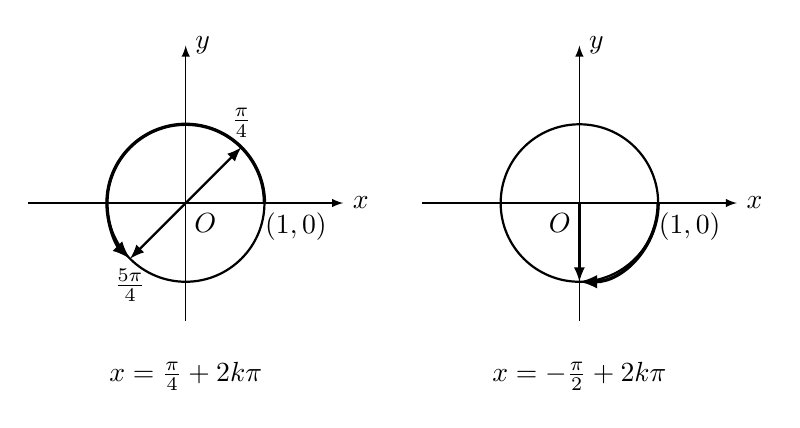
\begin{tikzpicture}[>=latex]
\begin{scope}
  \draw[->] (-2,0)--(2,0)node[right]{$x$};
  \draw[->] (0,-1.5)--(0,2)node[right]{$y$};
\draw[thick] (0,0) circle (1);
\draw[very thick,->] (1,0) arc (0:180+45:1);
\draw[thick, <->] (45:1)node[above]{$\frac{\pi}{4}$}--(180+45:1)node[below]{$\frac{5\pi}{4}$};
\node at (.25,-.25){$O$};
\node at (1.4,0)[below]{$(1,0)$};
\node at (0,-2.2){$x=\frac{\pi}{4}+2k\pi$};
\end{scope}
\begin{scope}[xshift=5cm]
  \draw[->] (-2,0)--(2,0)node[right]{$x$};
  \draw[->] (0,-1.5)--(0,2)node[right]{$y$};
  \draw[thick] (0,0) circle (1);
\draw[very thick,->] (1,0) arc (0:-90:1);
\draw[thick, ->] (0,0)--(-90:1);
\node at (-.25,-.25){$O$};\node at (1.4,0)[below]{$(1,0)$};
\node at (0,-2.2){$x=-\frac{\pi}{2}+2k\pi$};
\end{scope}
\end{tikzpicture}
  \caption{}
\end{figure}

显然(10.11)又可写成
\begin{equation}
  x=\frac{\pi}{4}+2k\pi
\end{equation}
和
\begin{equation}
  x=\frac{5\pi}{4}+2k\pi
\end{equation}
再由(10.12), (10.13), (10.14)容易看出角$3x$与角$-\frac{3\pi}{2}$, $\frac{3\pi}{4}$和$-\frac{\pi}{4}$
有相同的终边,所以若将式(10.12)和式(10.14)
代入$\sin3x$中,便得到
\[\begin{split}
  \sin 3\left(-\frac{\pi}{2}-2k\pi\right)&=\sin\left(-\frac{3\pi}{2}\right)=-\sin\frac{3\pi}{2}=1\\
  \sin 3\left(\frac{5\pi}{4}+2k\pi\right)&=\sin\frac{15\pi}{4}=\sin\left(4\pi-\frac{\pi}{4}\right)=\sin\left(-\frac{\pi}{4}\right)=-\frac{\sqrt{2}}{2}<0
\end{split}\]
因此这两组解是增解,应该舍去,经检验知
$x=\frac{\pi}{4}+2k\pi$满足不等式组, 
所以方程的解集是
$\left\{x\Big|x=\frac{\pi}{4}+2k\pi,\quad k\in\mathbb{Z}\right\}$








\end{solution}

\section*{习题10.4}
\begin{enumerate}
  \item 解下列各指数方程:
\begin{multicols}{2}
\begin{enumerate}
\item $3^{2 x-1}=81$
\item $\sqrt{5^{x}}=\sqrt[3]{25}$
\item  $\sqrt[4]{7^{x}}=\sqrt[5]{343}$
\item $\sqrt[4]{a^{x+1}}=\sqrt[3]{a^{x-3}}$

$(a>0,\;  a \neq 1)$
\item  $\sqrt{2^{x}} \sqrt{3^{x}}=36$
\item $\left(\frac{3}{4}\right)^x=\left(\frac{4}{3}\right)^5$
  \item $\left(\frac{4}{9}\right)^{4}=\left(\frac{3}{2}\right)^{x}$
  \item $\left(\frac{2}{3}\right)^{x}\left(\frac{9}{8}\right)=\frac{27}{64}$
  \item $ 4^{\sqrt{x+1}}=64 \cdot 2^{\sqrt{x+1}} $
  \item $(0.25)^{x-2}=\frac{256}{2^{x+3}}$
  \item  $\left(\frac{4}{9}\right)^{x}\left(\frac{27}{8}\right)^{x-1}=\frac{2}{3}$
  \item  $2^{x} \cdot 5^{4}=0.1\left(10^{x-1}\right)^{5}$
\end{enumerate}
\end{multicols}


\item  解下列各指数方程:
\begin{enumerate}
  \begin{multicols}{2}
\item $3^{x+2}+3^{x-1}=28$
\item  $5^{x+1}-5^{x-1}=24$
\item  $3^{2 x-1}+3^{2 x-2}-3^{2 x-4}=315$
\item  $3^{x}+3^{x+1}+3^{x+2}=5^{x+1}+5^{x+2}$
\item  $4^{x}+2^{x+1}=80$ 
\item  $ 3^{x+2}+9^{x+1}-810=0$
\item  $3^{2 x+5}=3^{x+2}+2$
\item   $3^{4 \sqrt{x}}-4.3^{2 \sqrt{x}}+3=0$
\item   $4.9^{\sqrt{x}-2}-3.15^{\sqrt{x}-2}=25^{\sqrt{x}-2} $
\item   $4^{2 x}-2.18^{2 x}=3.81^{28} $
\end{multicols}
\item   $\left(\sqrt{5+2 \sqrt{6}}\right)^{x}+\left(\sqrt{5-2 \sqrt{6}}\right)^{x}=\frac{10}{3}$
\end{enumerate}


\item  求最小整数指数 $x$, 使
\begin{multicols}{2}
  \begin{enumerate}
    \item  $\left(\frac{4}{5}\right)^{x}<0.000001$
  \item  $\left(\frac{3}{5}\right)^{x}<0.0001$
    \item $\left(\frac{10}{9}\right)^{x}>1000000$
    \item $\left(\frac{4}{5}\right)^{x}>10000000$
  \end{enumerate}
\end{multicols}

\item  解下列各不等式
\begin{multicols}{2}
\begin{enumerate}
 \item  $3^{3-5 x}-\frac{1}{81}>0$
\item  $(0.3)^{2 x^{2}+5 x+2}<1$
\item  $8^{x}+16^{\tfrac{3}{4} x+1}<34$
\item  $\frac{(0.5)^{3 x^{2}+10 x+6}}{100}<0.00125$
\item  $2^{x+1} \cdot 5^{2 x-3}<\frac{24}{25}$
\item  $5^{2x}-30.5^{x}+125<0$
\item  $2^{3 x}-2^{x+1}<2^{3} $
\item  $\frac{1}{\left(\frac{1}{10}\right)^{y}-1} \leqslant \frac{2}{\left(\frac{1}{100}\right)^{y}-10}$
\item  $\frac{1}{2^{x}-1} \geqslant \frac{1}{4^{x}-3}$
\item  $\left(\frac{3}{4}\right)^{x-2}\left(\frac{4}{3}\right)^{\tfrac{1}{x}}>\frac{9}{16}$
\end{enumerate}
\end{multicols}


\item  解下列各对数方程:

  \begin{enumerate}
   \item  $\lg x=2-\lg 5$
   \item $\lg(x+6)-\frac{1}{2}\lg(2x-3)=2-\lg 25$
 \begin{multicols}{2}
   \item $\frac{2\lg x}{\lg(5x-4)}=1$
   \item $\frac{\lg x}{1-\lg x}=2$
   \item $\log_{x-1}(x^2-5x+10)=2$
  \item  $2 \lg x=-\lg \left(6-x^{2}\right)$
  \item  $\frac{1}{5-\lg x}+\frac{1}{1+\lg x}=1$
  \item  $0.5 \lg (2 x-1)+\lg \sqrt{x-9}=1$
  \item  $\log _{2} \log _{3} \log _{4} x=0$
  \item  $\lg 9^{-1}+x \lg \sqrt[3]{3^{5 x-7}}=0$
  \item  $\lg 10^{\lg\left(x^{2}+21\right)}-1=\lg x$
  \end{multicols}   
  \end{enumerate}


\item 解下列各对数方程:
  \begin{enumerate}
  \item  $2 \log _{4} x+2 \log _{x} 4=5$ 
  \item  $\log _{2}(x-1)^{2}-\log _{0.5}(x-1)=9$
  \item  $\log _{8} x+\log _{4} x+\log _{2} x=7$
  \item  $\log _{x}\left(5 x^{2}\right) \cdot\left(\log _{5} x\right)^{2}=1$
  \item  $\sqrt{\log _{x} 5 \sqrt{5}+\log _{\sqrt{5}} 5 \sqrt{5}} \cdot \log _{\sqrt{5}} x=-\sqrt{6}$
  \item  $\sqrt{\log _{x} \sqrt{3 x}} \cdot \log _{3} x=-1$
  \item  $\log _{3 x}\left(\frac{3}{x}\right)+\log _{3}^{2} x=1$
  \item $\frac{\lg\left(\sqrt{x+1}+1\right)}{\lg\sqrt[3]{x-40}}=3$
  \end{enumerate}

  \item 解下列各方程:
\begin{enumerate}
  \item $(0.4)^{\lg^2 x+1}=(6.25)^{2-\lg x^3}$
  \item $x^{\lg x+2}=1000$
  \item $\sqrt{x^{\lg \sqrt{x}}}=10$
\item $\lg 2+\lg \left(4^{x-2}+9\right)=1+\lg \left(2^{x-2}+1\right)$
\item $\log _{2}\left(9^{x-1}+7\right)=2+\log _{2}\left(3^{x-1}+1\right)$
\item $\lg x+\lg \sqrt[3]{x}+\lg  \sqrt[9]{x}+\cdots=3$
\item $\log _{9} x+\left(\log _{9} x\right)^{2}+\left(\log _{9} x\right)^{3}+\cdots=1$,
\item $ 1+\log _{x} \frac{4-x}{x}=(\operatorname{lglg} n-1) \log _{x} 10$
\end{enumerate}

\item 解下列各方程组:
\begin{multicols}{2}
\begin{enumerate}
  \item  $\begin{cases}2^{\sqrt{{x}}+\sqrt{y}}=512 \\ \lg \sqrt{x y}=1+\lg 2\end{cases}$
\item  $\begin{cases}\log _{x} \log _{2} \log _{x} y=0 \\ \log _{y} 9=1\end{cases}$
\item  $\begin{cases}2^{\tfrac{x-y}{2}}-2^{\tfrac{x-y}{4}}=2 \\ 3^{\lg(2 y-x)}=1\end{cases}$
\item $\begin{cases}x y=40 \\ x^{12 y}=4,\end{cases}$
\item  $\begin{cases}3.2^{x}-\log _{2} y=2 \\ 2^{x} \cdot \log _{2} y=1\end{cases}$
\item  $\begin{cases}7^{y} \cdot \log _{5} x=2 \\ 4.7^{y}+\log _{5} x=2\end{cases}$
\item $\begin{cases}
\lg^2x+\lg^2y=5\\
\lg x-\lg y=1
\end{cases}$
\item 求$\begin{cases}
x^{x+y}=y^{12}\\
y^{x+y}=x^3
\end{cases}$的整数解
\end{enumerate}
\end{multicols}

\item 解下列各不等式:
\begin{enumerate}
  \begin{multicols}{2}
\item $\lg x>3$
\item $\lg (-x)>3$
\item $\lg x^2>3$
\item $\lg^2 x>3$
\item $\lg x<2\lg x$
\item $\lg x>2\lg x$
\item $\log_{\tfrac{1}{2}}(3x-5)<3$
\item $\lg x+\lg (x-3)>1$
\item $\lg (4x^2-9)>\lg (2x-3)+2$
\item $\lg (3-x)-1>\lg (2-x)$    
  \end{multicols}
\item $\log_{\sqrt{0.5}}(26x)>\log_{\sqrt{0.5}}(5x^2+5)$
\item $\log_{\sqrt{2}}(x^2-2x+8)+2\sqrt{\log_2(x^2-2x+8)}\ge 12$
\item $x^{\log_a x+1}>ax^2,\qquad (a>1)$
\end{enumerate}

\item 求解
\begin{enumerate}
  \item 试求满足不等式$2(\log_{0.5}x)^2+9\log_{0.5}x+9\le 0$的$x$的范围;
  \item $x$在1中求得的范围内变动时,试求
$f(x)=\left(\log_2 \frac{x}{3}\right)\left(\log_2 \frac{x}{4}\right)$
的最大值$M$和最小值$L$.
\end{enumerate}

\item 解下列方程:
\begin{multicols}{2}
  \begin{enumerate}
  \item $\log_{\sqrt{2}\sin x}(1+\cos x)=2$
  \item $\log_{\tfrac{1}{8\cos^2 x}}\sin x=\frac{1}{2}$
  \item $\frac{2}{\lg\left(\frac{1}{2}+\cos^2 x\right)}=\log_{\sin 2x}10$
  \item $\arcsin(\lg x)=0$
  \item $\lg(\arcsin x)=0$
  \item $\arccos(\pi\log_3\tan x)=0$
\end{enumerate}
\end{multicols}

\end{enumerate}